\documentclass[../main-sheet.tex]{subfiles}
\usepackage{../style}
\graphicspath{ {../img/} }
\backgroundsetup{contents={}}
\begin{document}
\section{Predictor-Corrector Method}
\underline{Remainder:}\\
Adams-Bashforth four-step method:
\begin{align*}
    w_0&=\alpha, \quad w_1=\alpha_1,\quad w_2=\alpha_2,\quad w_3=\alpha_3\\
    w_{i+1}&=w_i+\frac{h}{24}\left[ 55f(t_i,w_i)-59f(t_{i-1},w_{i-1})+37f(t_{i-2},w_{i-2})-9f(t_{i-3},w_{i-3}) \right]\quad\text{ for } i=3,4,5,\dots, N-1
\end{align*}
Adams-Moulton three-step method:
\begin{align*}
    w_0&=\alpha, \quad w_1=\alpha_1,\quad w_2=\alpha_2\\
    w_{i+1}&=w_i+\frac{h}{24}\left[ 9f(t_{i+1},w_{i+1})+19f(t_{i},w_{i})-5f(t_{i-1},w_{i-1})+f(t_{i-2},w_{i-2}) \right]\quad\text{ for } i=2,3,\dots, N-1
\end{align*}
IVP: \(\ddt{y}=y'=f(t,y);\quad a\leq t\leq b, y(a)=y(t_0)=\alpha\)\\
For \(i=3\), from Adams-Bashforth four-step method, we have,
\begin{equation}
    w_{4}=w_3+\frac{h}{24}\left[ 55f(t_3,w_3)-59f(t_{2},w_{2})+37f(t_{1},w_{1})-9f(t_{0},w_{0}) \right]\label{eq:pred1}
\end{equation}
For Predictor-Corrector method, we denote \(w_4^{(0)}\) for \(w_4\) so 
\begin{equation}
    w_{4}^{(0)}=w_3+\frac{h}{24}\left[ 55f(t_3,w_3)-59f(t_{2},w_{2})+37f(t_{1},w_{1})-9f(t_{0},w_{0}) \right]\label{eq:pred2}
\end{equation}
Here we know only \(w_0=\alpha\), so, first we need to calculate \(w_1\), \(w_2\), \(w_3\) using RK-4. Then using the values of \(w_0\), \(w_1\), \(w_2\), \(w_3\) we will get \(w_4^{(0)}\) from \eqref{eq:pred2}.\\
Now, we use Adams-Moulton three-step method as a corrector:
\begin{equation}
    w_{4}^{(1)}=w_3+\frac{h}{24}\left[ 9f(t_{4},w_{4}^{(0)})+19f(t_{3},w_{3})-5f(t_{2},w_{2})+f(t_{1},w_{1}) \right]\label{eq:pred3}
\end{equation}
Here \(f(t_4,w_4^{(0)})\) will evaluate using the value of \(w_4^{(0)}\) that already calculated using \eqref{eq:pred2}.\\
After calculation of \eqref{eq:pred3}, we will get \(w_4^{(1)}\). If we will not achieve required accuracy, e.g., \(\abs{w_4^{(1)}-w_4^{(0)}}<10^{-4}\), then we have to proceed in the following way:
\begin{equation}
    w_{4}^{(2)}=w_3+\frac{h}{24}\left[ 9f(t_{4},w_{4}^{(1)})+19f(t_{3},w_{3})-5f(t_{2},w_{2})+f(t_{1},w_{1}) \right]\label{eq:pred4}
\end{equation}
Note that only \(f(t_4,w_4^{(1)})\) have to evaluate but \(f(t_3,w_3)\), \(f(t_2,w_2)\), \(f(t_1,w_1)\) already evaluated when you perform equation \eqref{eq:pred2}.\\
If \(w_4^{(2)}\) is not achieved desired accuracy, then 
\begin{equation}
    w_{4}^{(3)}=w_3+\frac{h}{24}\left[ 9f(t_{4},w_{4}^{(2)})+19f(t_{3},w_{3})-5f(t_{2},w_{2})+f(t_{1},w_{1}) \right]\label{eq:pred5}
\end{equation}
If still not get required accuracy, we will have to repeat these processes.\\
If required accuracy will achieve (say \(w_4^{(0)}\) or \(w_4^{(1)}\) or \(w_4^{(2)}\) or \(w_4^{(3)}\)), then 
\begin{equation}
    w_{5}^{(1)}=w_4+\frac{h}{24}\left[ 9f(t_{5},w_{5}^{(0)})+19f(t_{4},w_{4})-5f(t_{3},w_{3})+f(t_{2},w_{2}) \right]\label{eq:pred6}
\end{equation}
where,
\begin{equation}
    w_{5}^{(0)}=w_4+\frac{h}{24}\left[ 55f(t_4,w_4)-59f(t_{3},w_{3})+37f(t_{2},w_{2})-9f(t_{1},w_{1}) \right]\label{eq:pred7}
\end{equation}
[Here \(w_4\) is either \(w_4^{(0)}\) or \(w_4^{(1)}\) or \(w_4^{(2)}\) or \(w_4^{(3)}\)]\\
Equation \eqref{eq:pred6} is repeated until get required accuracy.
\begin{ex}
    IVP: \(y'=y-t^2+1\); \(0\leq t\leq 2\), \(y(0)=0.5\) and \(N=10\), so \(h=0.2\).
    \begin{center}
        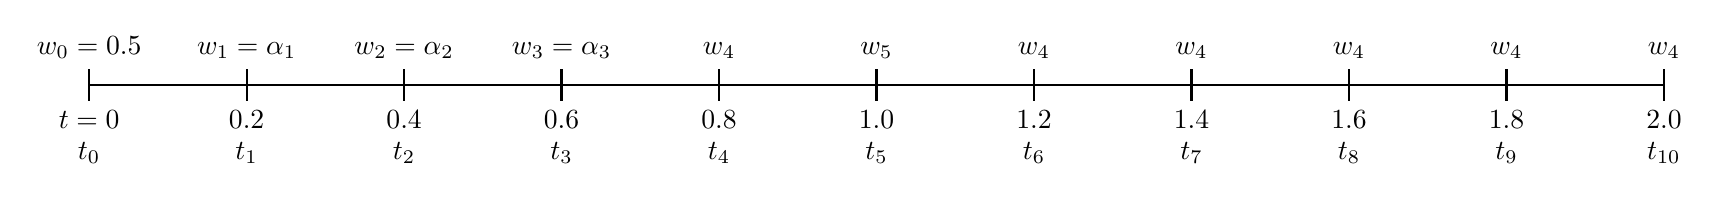
\begin{tikzpicture}
            \draw[solid,thick] (0,0) -- (20,0);
            \draw[thick] (0,0.2)node[above] {$w_0=0.5$} -- ++ (0,-0.4) node[below] {$t=0$} (0,-0.6) node[below] {$t_0$};
            \draw[thick] (2,0.2)node[above] {$w_1=\alpha_1$} -- ++ (0,-0.4) node[below] {$0.2$}(2,-0.6) node[below] {$t_1$};
            \draw[thick] (4,0.2)node[above] {$w_2=\alpha_2$} -- ++ (0,-0.4) node[below] {$0.4$}(4,-0.6) node[below] {$t_2$};
            \draw[thick] (6,0.2)node[above] {$w_3=\alpha_3$} -- ++ (0,-0.4) node[below] {$0.6$}(6,-0.6) node[below] {$t_3$};
            \draw[thick] (8,0.2)node[above] {$w_4$} -- ++ (0,-0.4) node[below] {$0.8$}(8,-0.6) node[below] {$t_4$};
            \draw[thick] (10,0.2)node[above] {$w_5$} -- ++ (0,-0.4) node[below] {$1.0$}(10,-0.6) node[below] {$t_5$};
            \draw[thick] (12,0.2)node[above] {$w_4$} -- ++ (0,-0.4) node[below] {$1.2$}(12,-0.6) node[below] {$t_6$};
            \draw[thick] (14,0.2)node[above] {$w_4$} -- ++ (0,-0.4) node[below] {$1.4$}(14,-0.6) node[below] {$t_7$};
            \draw[thick] (16,0.2)node[above] {$w_4$} -- ++ (0,-0.4) node[below] {$1.6$}(16,-0.6) node[below] {$t_8$};
            \draw[thick] (18,0.2)node[above] {$w_4$} -- ++ (0,-0.4) node[below] {$1.8$}(18,-0.6) node[below] {$t_9$};
            \draw[thick] (20,0.2)node[above] {$w_4$} -- ++ (0,-0.4) node[below] {$2.0$}(20,-0.6) node[below] {$t_{10}$};
            \end{tikzpicture}
    \end{center}
    For Predictor-corrector process; here \(w_0=\alpha=0.5\) is known, so we have to evaluate \(w_1\), \(w_2\), \(w_3\) with RK4, then using these values, we will get \(w_4^{(0)}\) from \eqref{eq:pred2}. After getting \(w_4^{(0)}\), we will obtain \(w_4^{(1)}\) using \eqref{eq:pred3}.

    \(w_4^{(1)}\) is the approximate value at \(t=t_4=0.8\). Such process is needed to repeat until \(t=t_{10}=2\).
\end{ex}
\begin{note}
    \[w_{i+1}^{(k+1)}=w_i+\frac{h}{24}\left[ 9f(t_{i+1},w_{i+1}^{(k)})+19f(t_{i},w_{i})-5f(t_{i-1},w_{i-1})+f(t_{i-2},w_{i-2}) \right]\]
    Here `\(k\)' is the iteration index and \(i\) is the grid/node index.\\
    Let \(k=0\); then,
    \[w_{i+1}^{(1)}=w_i+\frac{h}{24}\left[ 9f(t_{i+1},w_{i+1}^{(0)})+19f(t_{i},w_{i})-5f(t_{i-1},w_{i-1})+f(t_{i-2},w_{i-2}) \right];\quad i=3,4,5,\dots\]
    So,
    \[w_{4}^{(1)}=w_3+\frac{h}{24}\left[ 9f(t_{4},w_{4}^{(0)})+19f(t_{3},w_{3})-5f(t_{2},w_{2})+f(t_{1},w_{1}) \right]\]
    which is equation \eqref{eq:pred3}.\\
    If \(i=4\), then we will get equation \eqref{eq:pred6} and so on.\\
    If we put \(k=1\) and \(i=3\), then we will get equation \eqref{eq:pred4} and so on.
\end{note}
\end{document}